\section{Schnittstellen}
\label{sec:Kap-8.6}

Die generische (in vielen Programmiersprachen sagt man öffentliche) Schnittstelle einer Klasse ist das, was diese nach außen für Dienstnutzer sichtbar macht. Wenn ein Dienstnutzer direkt auf den Attributen der Klasse arbeiten würde, würde das Kapselungsprinzip der Objektorientierung verletzt. Denn auf den Daten (Attributen) einer Klasse sollen nur seine eigenen Operationen arbeiten dürfen. Die Attribute einer Klasse sollten also für Objekte anderer Klassen nicht direkt zugänglich sein. Man steuert das in der konkreten Programmierung durch sogenannte Sichtbarkeiten (s. Lektion~6). Gleiches kann die Klasse auch für ihre Operationen anwenden, nämlich diejenigen unsichtbar nach außen halten, die nicht aufgerufen werden sollen. Was dann übrigbleibt ist die Menge von Operationen, die durch Dienstnutzer aufgerufen werden können, um die Funktionalität des Gesamtsystems zu gewährleisten. Diese bilden die generische Schnittstelle der Klasse. Zur Wahrung des Geheimnisprinzips genügt die generische Schnittstelle einer Klasse.

Weitergehende Entwurfsprinzipien, wie die aus Abschnitt~\ref{sec:Kap-7.2}, setzen statt auf die generische auf explizit spezifizierte eigenständige Schnittstellen. In der UML und in vielen Programmiersprachen heißt dieses Konzept nach der englischen Bezeichnung für Schnittstelle \textit{Interfaces}. Man formuliert -- ein wenig verwirrend --, dass ein Interface eine Schnittstelle zu einer (oder auch mehreren) Klasse(n) \textbf{bildet} und dass aus Sicht der Klasse gesehen, diese das Interface \textbf{realisiert}. In manchen Programmiersprachen formuliert man auch, die Klasse \textbf{implementiert} das Interface, Java zum Beispiel nutzt das Schlüsselwort implements.

\vspace{\baselineskip} %%% für Druck

\begin{figure}[h!]
	\centering
	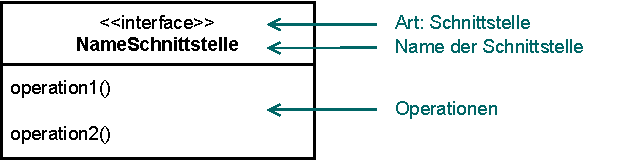
\includegraphics[scale=1.0]{Bilder/Kapitel-8/schnittstelle_in_uml.pdf}
	\caption{Darstellung eines Interfaces in UML}
	\label{fig:schnittstelle_in_uml}
\end{figure}

\vspace{\baselineskip} %%% für Druck

Interfaces haben eine ähnliche Wirkungsweise wie abstrakte Klassen: Sie machen Vorgaben für das Vorhandensein von Operationen in den Klassen, die das Interface realisieren. Abbildung~\ref{fig:schnittstelle_in_uml} zeigt die UML-Darstellung eines Interfaces. 

Wie bei den abstrakten Operationen einer abstrakten Klasse wird bei den Operationen im Interface nur der Operationskopf angegeben. Vom Konzept her haben Interfaces zudem keine Attribute, in manchen Programmiersprachen kann ein Interface aber Konstanten mit vorgeben. Ebenso wie bei abstrakten Klassen können von Interfaces keine Instanzen gebildet werden. Im Unterschied zu abstrakten Klassen müssen bei Interfaceverwendung die Klassen, die ein Interface realisieren, nicht in einer Vererbungshierarchie stehen. Jede Klasse des Softwaresystems könnte jedes beliebige vorhandene Interface realisieren, indem sie die dort vorgegebenen Opera\-tionen anbietet -- inhaltlich macht das natürlich keinen Sinn. Eine Klasse kann auch mehrere Interfaces realisieren. Auf diese Weise wird zum Beispiel Mehrfach\-vererbung in Programmiersprachen realisiert, die das Konzept Mehrfachvererbung nicht vor\-sehen.

\vspace{\baselineskip} %%% für Druck

\begin{figure}[h!]
	\centering
	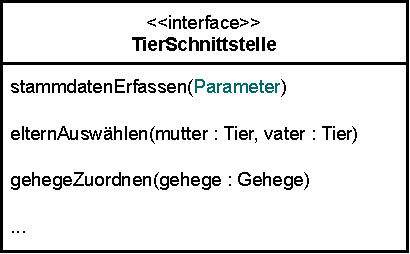
\includegraphics[scale=1.0]{Bilder/Kapitel-8/interface_tier.pdf}
	\caption{Interface \sttpUMLText{Tier}}
	\label{fig:interface_tier}
\end{figure}

\vspace{\baselineskip} %%% für Druck

Abbildung~\ref{fig:interface_tier} zeigt ein Interface für die Tier-Klasse von Seite~\pageref{sec:Kap-8.2:Tierklasse}, das speziell auf die Tätigkeiten zugeschnitten ist, die der Tierpfleger bei der Erfassung neu\-geborener Tiere ausführen soll. In der Operation \sttpUMLText{stammdatenErfassen()} steht in der Abbildung nur ein Platzhalter „Parameter“. Je nachdem, welche der Attribute der Klasse \sttpUMLText{Tier} zu den Stammdaten gezählt werden, können dort unterschiedlich viele Parameter aufgeführt werden. Folgt man der textuellen Beschreibung auf Seite~\pageref{sec:Kap-8.2:Tiererfassung} sind das Name, Größe, Geburtsdatum und Gewicht.

\vspace{\baselineskip} %%% für Druck

\begin{figure}[h!]
	\centering
	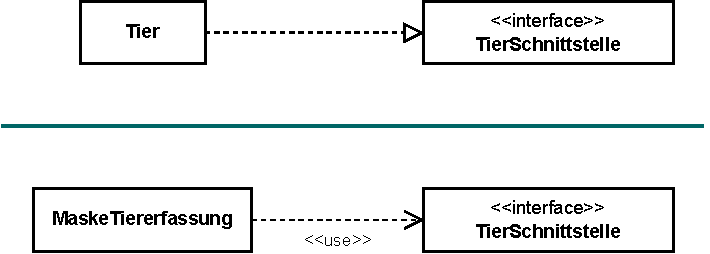
\includegraphics[scale=1.0]{Bilder/Kapitel-8/schnittstellen_verwendung.pdf}
	\caption{Schnittstellenverwendung}
	\label{fig:schnittstellen_verwendung}
\end{figure}  

\vspace{\baselineskip} %%% für Druck

Abbildung~\ref{fig:schnittstellen_verwendung} zeigt, wie die Verwendung von Schnittstellen in UML modelliert wird. In dem oberen Teil der Abbildung ist dargestellt, dass die Klasse \sttpUMLText{Tier} das Interface \sttpUMLText{TierSchnittstelle} realisiert. Der untere Teil der Abbildung zeigt die UML-Syntax, wenn eine Dienstnutzerklasse das Interface verwendet, um die entsprechenden Funktionalitäten der Klasse \sttpUMLText{Tier} zu nutzen.



